\chapter{Multi-agent reinforcement learning} \label{ch:marl}

\begin{chapter_outline}

In this chapter, we provide a broader overview of reinforcement learning.
We first introduce reinforcement learning in Section \ref{sec:ch2_Introduction} and define a stochastic game, the most common multi-agent framework, in Section \ref{sec:ch2_stochastic_Game}.
Multi-agent reinforcement learning is commonly divided into three settings, based on the relative goals of agents, and described in Section \ref{sec:ch2_multi_agent_settings}.
When there is a single agent, we are in the particular case called single-agent reinforcement learning.
In \ref{sec:ch2_single_agent_RL}, we provide essential details on this (not so) particular case where the foundations of multi-agent approaches reside.
Following this, a discussion on partial-observability is pursued in Section \ref{sec:ch2_partial_observability}.
In the last Section \ref{sec:ch2_futher}, we present readings of interest to go further on the topics broadly introduced in this Chapter.

\end{chapter_outline}

\section{Introduction} 
\label{sec:ch2_Introduction}
Reinforcement learning (RL) is a machine learning (ML) setting to solve decision-making problems.
We hereafter paraphrase several RL definitions.
Reinforcement learning is learning solutions of a sequential decision process by repeatedly interacting with an environment \citep{marl-book}.
Reinforcement learning is a kind of ML where an agent has to learn how to interact with its environment. \citep{pml1Book}.
Reinforcement learning is a framework for sequential decision-making, one core topic of ML \citep{introDeepRL}.
Reinforcement learning is a method to solve problems where decisions are applied to a system over time to achieve a desired goal \citep{BusoniuErnstBook}.
Reinforcement learning is learning by interacting in its environment to maximise a numerical signal called reward \citep{sutton2018reinforcement}.

In this 

multi-agent vs single-agent
Deep RL

define MARL and SARL

\section{Stochastic game}
\label{sec:ch2_stochastic_Game}
The stochastic game \citep{stochasticGames} is probably the most general framework in multi-agent.
In a stochastic game, a set of agents interact with the environment by observing the state of the environment, choosing actions and receiving rewards over a sequence of time, finite or not.
In this manuscript, we define a stochastic game by a tuple $[n, \mathcal{S}, \mathcal{U}, R, P, \gamma]$.
An agent is represented by $a$, and the set of agents is $\mathcal{A} \equiv \{1,..,n\}$.
We thus define each agent as $a_i$ with $i \in \mathcal{A}$ and any agent by $a$.

\todo: check state space vs set of 

At each time step $t$, each agent $a$ observes the state of the environment $s_t \in \mathcal{S}$ and selects an action $u_t^a \in \mathcal{U}^a$ with a probability given by its policy $\pi^a(u_t|s_t)$, where $\mathcal{S}$ is the state space, and $\mathcal{U}^a$ is the action space of agent $a$.
The joint action space is thereby $\mathcal{U} \equiv \bigtimes_{i \in \mathcal{A}} \mathcal{U}^{a_i}$, the joint action is $\mathbf{u} \in \mathcal{U}$ and the joint policy is $\mathbf{\pi}$.
As a consequence of the $n$ selected actions, the state of the environment $s_t$ transits to a new state $s_{t+1}$ with a probability $P(s_{t+1}, s_t, \mathbf{u_t})$ defined by the transition function $P:\mathcal{S} \times \mathcal{S} \times \mathcal{U} \rightarrow [0,1]$.

As the state transitions, each agent receives a reward denoted $r_t^{a_i} = R(s_{t+1}, s_t, \mathbf{u_t}, i)$ and defined by the reward function $R: \mathcal{S} \times \mathcal{S} \times \mathcal{U} \times \mathcal{A} \rightarrow \mathbb{R}$.
The goal of each agent $a_i$ is to maximise its expected sum of discounted rewards $\mathbb{E}_{\mathbf{\pi}}\left[ \sum_{t=0}^{T-1} \gamma^t r^{a_i}_t \right]$, where $T$ is the time horizon and $\gamma \in ]0, 1]$ the discount factor.
It is worth enforcing that the reward received by an agent is thus a function of the joint policy and not only of its policy.
The time horizon $T$, considered finite, defines the length of an episode, which is a complete sequence of actions in the environment.
Finally, the discount factor $\gamma$ defines the importance of future reward.

Finding or learning the optimal policy that maximises this expected sum is the purpose of reinforcement learning.
One solution to a stochastic game is to find a Nash equilibrium.
\todo: nash equilibrium

Several comments can be addressed in the context of the works presented in this manuscript.
In the stochastic game definition, some include an initial state $s_0$ distribution which we keep implicit (e.g. \citep{marl-book}).
While the state space can be composed of discrete or continuous variables, the action spaces are considered discrete.
Agents do not always observe the entire state of the environment to select an action.
This partial observability is further developed in Section \ref{sec:ch2_partial_observability}.
In the literature, a stochastic game is sometimes called a Markov game (e.g. \citep{MarkovGames}).

\section{Multi-agent settings} 
\label{sec:ch2_multi_agent_settings}
The stochastic game definition proposed in Section \ref{sec:ch2_stochastic_Game} provides a general framework for multi-agent systems.
By modifying the definition, it is possible to distinguish three main setting types hereafter briefly described: cooperation, competition and general sum game.
In Section \ref{sec:ch2_single_agent_RL}, we develop details about a particular case, the single-agent setting.

\subsection{Cooperation} 
\label{sec:ch2_Cooperation}
When agents share the same goal, they cooperate.
Sharing the same goal means that a single reward function can be used instead of a set of reward functions \citep{}.
This adaptation of a stochastic game is one solution, and Part \ref{part:coop} of this manuscript is dedicated to cooperative settings with a common reward.
\todo: find another type of solution

Many problems can be modelled as a cooperative multi-agent setting.
\todo: cooperative examples
Find nice examples for the different mode of training and execution.

\subsection{Competition} 
\label{sec:ch2_Competition}
When agents share opposite goals, they compete.
In competition, any action that benefits one agent incurs a retrofit to other ones.
This setting is often called a zero-sum game \citep{}.
The property of a zero-sum game is that all rewards sum to zero at any time.
In a two-agent zero-sum game, commonly known as a two-player zero-sum in the game theory literature \citep{}, a possible adaptation of the stochastic game is to have a single reward function that one tries to maximise while the other tries to minimise it.

Many problems can be modelled as a competitive multi-agent setting.
\todo: compet example



\subsection{General sum game} 
\label{sec:ch2_general_sum_game}
The third setting includes everything that is not purely cooperative or purely competitive.
In this manuscript, we are interested in the mixed cooperative-competitive setting where two teams compete against each other.
Part \ref{part:compet} is dedicated to these settings to study how competition methods work in accordance with cooperation ones.
\todo We can find several examples of such mixed cooperative-competitive settings.


Other general sum games exist, for example, when several agents have their interests but share the environment with others.

\todo traffic...


\section{Single-agent reinforcement learning} 
\label{sec:ch2_single_agent_RL}
As introduced, single-agent reinforcement learning (SARL) is the particular case of a multi-agent environment with a single agent.
Presented as such is a bit of a joke since the foundation of MARL relies on many works first proposed for single-agent environments.
In this section, we introduce the Markov decision process and discuss some fundamentals of RL.

\subsection{Markov decision process} \label{sec:ch2_mdp}
\begin{figure}
    \centering
    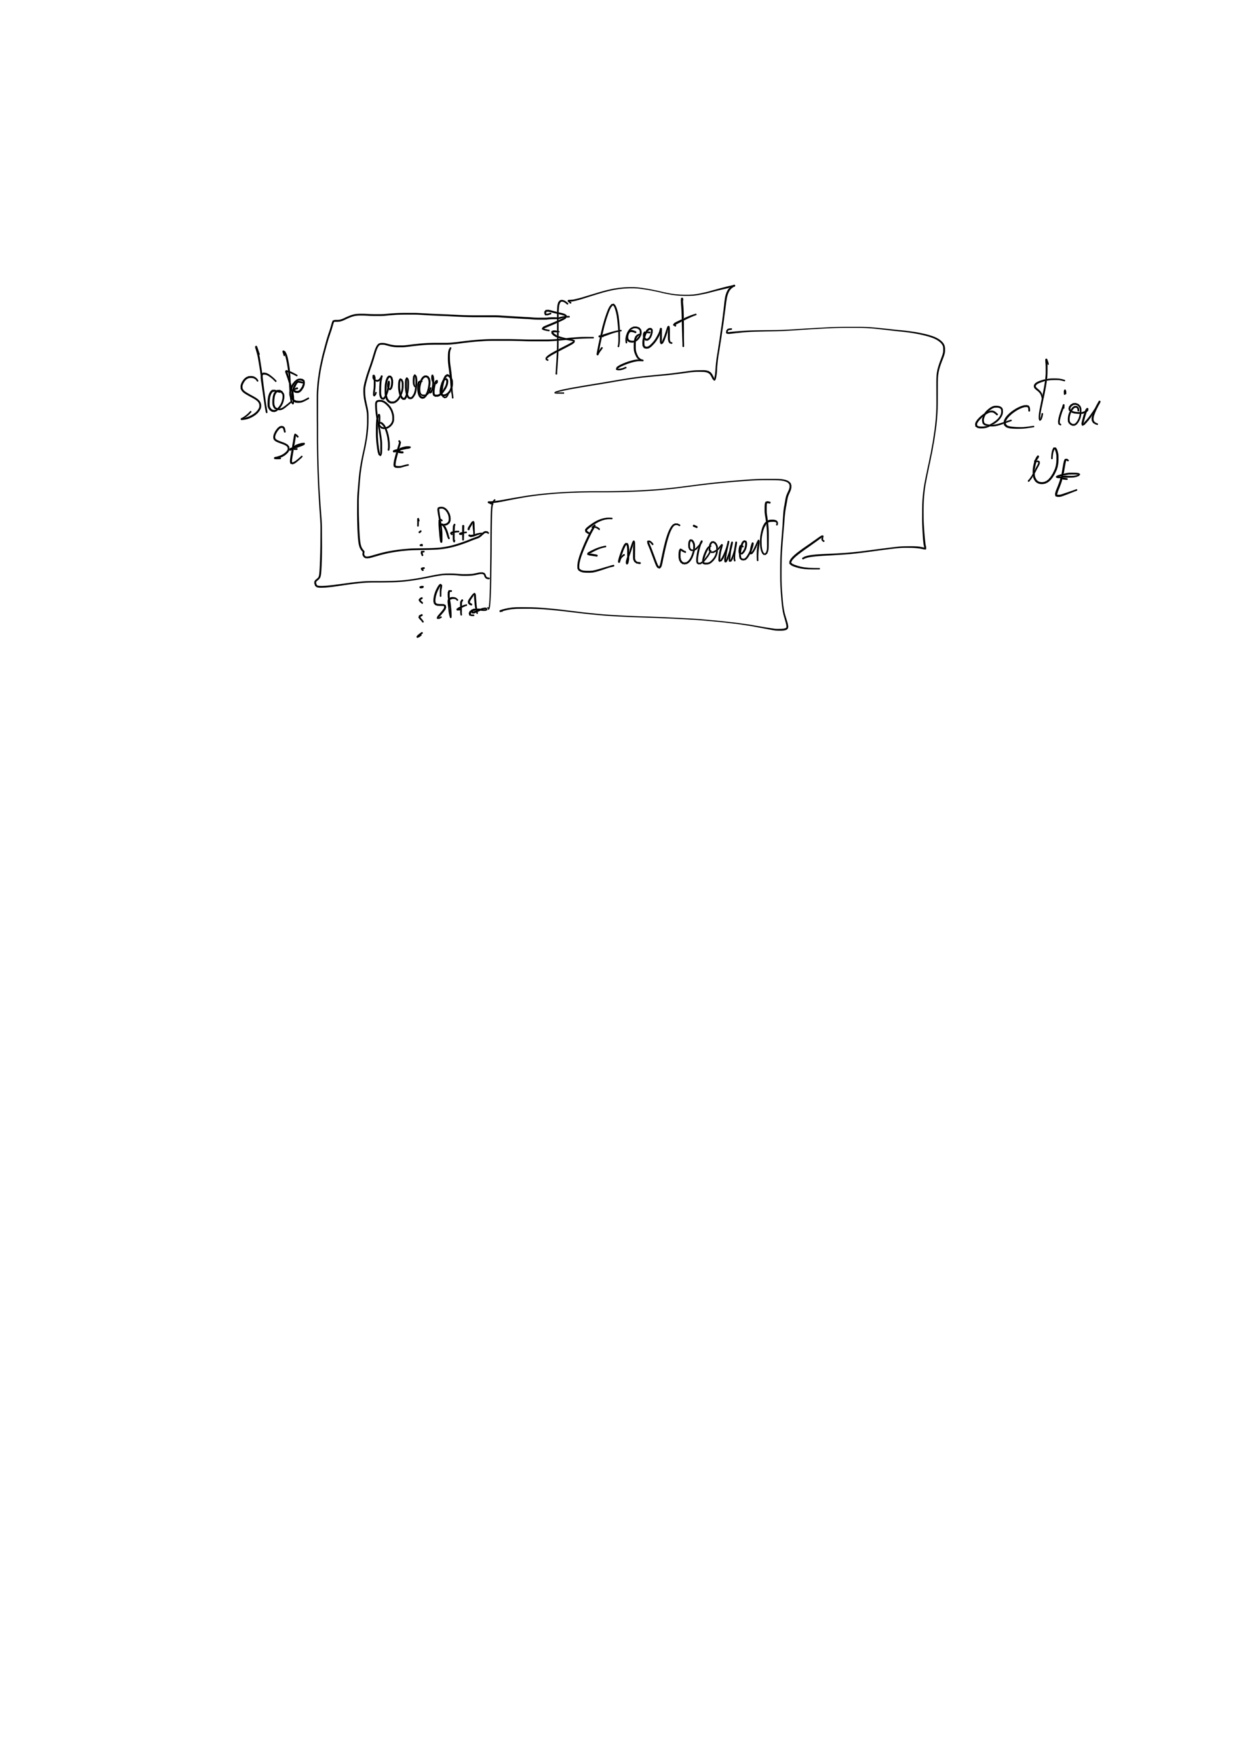
\includegraphics[width=\textwidth]{tex_thesis/figures/ch2/mdp_sketch.pdf}
    \caption{Markov decision process \citep{sutton2018reinforcement}. \todo check on the same page as the section where it is defined.}
    \label{fig:ch2_mdp}
\end{figure}

By removing the agents of the stochastic game definition of Section \ref{sec:ch2_stochastic_Game}, we obtain the definition of a Markov decision process (MDP).
We define an MDP as a tuple $[\mathcal{S}, \mathcal{U}, R, P, \gamma, p_0]$ where a single-agent interacts with its environment as presented in Figure \ref{fig:ch2_mdp}.
The agent of an MDP observes the state $s_t \in \mathcal{S}$ and selects an action from its action space $u_t \in \mathcal{U}$ with a probability defined by its policy $\pi(u_t|s_t)$.
This selected action leads the agent to a new state $s_{t+1}$ with a probability given by the transition function $P:\mathcal{S} \times \mathcal{S} \times \mathcal{U} \rightarrow [0,1]$.
Along the transition of the state, the agent receives a reward $r_t$ defined by the reward function $R:\mathcal{S} \times \mathcal{S} \times \mathcal{U} \rightarrow \mathbb{R}$.

We define the discounted return of a sequence from time step $t$ to time step $T$ as $G_t= \sum_{j=t}^{T-1} \gamma^j r_{t+j}$.
The goal of the agent is again to maximise the expected discounted return, so the expected sum of discounted rewards, over a finite episode $\mathbb{E}_{\pi} \left[\sum_{t=0}^{T-1} \gamma^t r_t \right]$, also denoted $\mathbb{E}_{\pi, p_0}\left[ G_0 \right]$ where $p_0$ is the initial distribution of $s_0$.
Therefore, it needs to find an optimal policy $\pi^*=\argmax_\pi \mathbb{E}_{\pi}\left[ G_0 \right]$.
To evaluate a policy, we define the state value function $V^\pi(s) = \mathbb{E}_{\pi}\left[G_t|s_t=s\right]$ and the state action value function $Q^\pi(s, u) = \mathbb{E}_{\pi}\left[G_t|s_t=s, u_t=u\right]$.

\todo: Markovian property.

\todo: deterministic policy.

\todo: The particular case of a Nash Equilibrium with a single agent.

Most commonly, two families of methods are identified in RL.
The value-based methods aim at learning a value function and derive the policy from it, while the policy-based methods directly learn a policy.

\subsection{Model-based or model-free}
\label{sec:ch2_model_based_vs_model_free}
When it comes to finding the optimal policy in an MDP, we distinguish methods based on the knowledge of action outcomes.
Indeed, with the model of the MDP, one can simulate the environment to evaluate policies \citep{sutton2018reinforcement}.
\cite{moerland2023model} defines it as `a model is a form of reversible access to the MDP dynamics (known or learned)'.
In RL, knowing the model and finding the optimal solution, or learning the model to use it to find the optimal solution, is referred to as model-based RL.
The opposite of learning by trial and error, without a model, is named model-free RL, and in this manuscript, we focus on model-free RL.

While model-based RL is not our primary focus, we hereafter discuss the notion of planning and highlight differences with model-free RL.
We try to identify definitions of planning based on the work of \cite{moerland2023model} and \cite{sutton2018reinforcement}.

\todo modelbased finish paragraph

\subsection{Dynamic programming}
Dynamic programming \citep{bellman1966dynamic} methods compute the optimal policy given a model of an MDP \citep{sutton2018reinforcement}.
They rely on the property that the value functions $V^{\pi^*}$ and $Q^{\pi^*}$ of the optimal policy ${\pi^*}$ satisfy the Bellman equations $\forall s, u$:
\begin{equation}
\label{eq:ch2_bellmanV}
    V^{\pi^*}(s) = \max_u \mathbb{E}[r_t + \gamma V^{\pi^*}(s_{t+1})| s_t=s, u_t=u]
\end{equation}

\begin{equation}
\label{eq:ch2_bellmanQ}
    Q^{\pi^*}(s, u) = \mathbb{E}[r_t + \gamma \max_{u'} Q^{\pi^*}(s_{t+1}, u') |s_t=s, u_t=u]
\end{equation}

Not going into the details of policy evaluation, policy improvement, policy iteration and value iteration, e.g. presented in \citep{sutton2018reinforcement}, one can find the optimal policy by iteratively evaluating and improving the policy with the value functions.
This can be highlighted by developing the value functions for any policy $\pi$ and $\forall s, u$:
\begin{equation}
\label{eq:ch2_V_2}
\begin{split}
    V^\pi(s)= \mathbb{E}_{\pi}\left[G_t|s_t=s\right] & = \mathbb{E}_{\pi}\left[r_t + \gamma V^\pi(s_{t+1})|s_t=s\right]\\
     & = \sum_{u} \pi(u|s) \sum_{s'} P(s', s, u) (R(s', s, u) + \gamma V^\pi(s'))
\end{split}
\end{equation}

\begin{equation}
\label{eq:ch2_Q_2}
\begin{split}
    Q^\pi(s, u) = \mathbb{E}_{\pi}\left[G_t|s_t=s, u_t=u\right] & = \mathbb{E}_{\pi}\left[r_t + \gamma V^\pi(s_{t+1})|s_t=s, u_t=u \right] \\
    &  = \sum_{s'} P(s', s, u) (R(s', s, u) + \gamma V^\pi(s'))
\end{split}
\end{equation}

In addition to requiring the model knowledge $P$ and $R$, the complexity of these methods increases with the size of the state space, often referred to as the curse of dimensionality, which may limit their usage.
Anyway, because of our direction towards model-free RL, our interest relies here on the presentation of Equations \ref{eq:ch2_bellmanV}, \ref{eq:ch2_bellmanQ}, \ref{eq:ch2_V_2} and \ref{eq:ch2_Q_2} that may ease the understanding of the learning concepts.


\subsection{Value-based methods} \label{sec:ch2_value_based_methods}
Value-based methods essentially learn value functions.
Maybe one of the first methods in model-free RL is Q-learning \citep{watkins1992q}, where the state-action value function learned is the optimal one defined as $Q^{\pi^*}(s, u)=\max_{\pi}Q^\pi(s, u)$.
This enables the agent to greedily select the action $\pi^*(u|s)=\argmax_u Q^{\pi^*}(s, u)$.

This is a tabular method as the idea of Q-learning is to maintain a table of estimations of $Q(s, u)$ and to update each estimation based on an other one, which is called bootstrapping.
This method is based on the idea called temporal difference (TD) learning.
Following the update rule of Equation \ref{eq:ch2_QLearning}, one can repeatedly update the estimation $Q(s, u)$ by adding the temporal difference weighted by a factor $\alpha$.

\begin{equation}
\label{eq:ch2_QLearning}
    Q(s_t, u_t) \leftarrow Q(s_t, u_t) + \alpha \left[ r_t + \gamma \max_u Q(s_{t+1}, u) - Q(s_t, u_t) \right]
\end{equation}

It is important to denote that this algorithm allows to approximate $Q^{\pi^*}(s, u)$ indepentely of the policy used to generate the transition ($s_t, u_t, r_t, s_{t+1}$).
Samples are typically generated with an $\epsilon$-greedy policy, that takes a random action instead of the greedy one with a probability $\epsilon$.
This is a characteristic of the off-policy methods, whereas the on-policy methods improves the policy used to generate the transitions.
In this manuscript, we consider only off-policy value-based methods but some on-policy methods are discussed further with policy-based methods.
SARSA is a well-known on-policy value-based method, e.g. in \citep{sutton2018reinforcement}.

With Q-learning, the table size to maintain increases as the state-action space size increases.
Therefore, it becomes impractical to compute $Q(s, u)$ for each state-action pair, and it requires function approximators.
There exist various function approximators, but here, we consider neural networks.
A neural network is a function $f: \mathcal{X} \rightarrow \mathcal{Y}$ that maps an input to an output based on its parameters $\theta$: $y = f(x;\theta)$.
Not going into the details, a neural network is commonly composed of a sequence of non-linear transformations of the input to compute the output.
The parameters are updated in order to minimise a loss function $\mathcal{L}(\theta)$ by gradient descent: $\theta = \theta - \alpha \nabla \mathcal{L}(\theta)$.
The loss function $\mathcal{L}(\theta)$ can be seen as a distance between the output $y$ and the prediction of the neural network $f(x;\theta)$.
\todo{ref neural net}

A solution, commonly referred to as deep Q-network (DQN) \citep{Mnih2015}, approximates $Q(s, u)$ with a neural network $\theta$ and learns $Q(s, u;\theta)$ by minimising the loss defined in Equation \ref{eq:ch2_dqnloss} where $B$ is a replay buffer and $\theta'$ is the target network.
The replay buffer $B$ stores transitions $\langle s_{t},u_{t},r_{t},s_{t+1}\rangle$ and the network $\theta$ is updated by sampling batches from it \citep{lin1992self}.
\todo{This allows updating the neural network with past transitions.}
The target network $\theta'$ is a copy of $\theta$ updated periodically.
This reduces the moving target problem as $\theta$ is updated several times before it is copied in $\theta'$ to update the target.

\begin{equation}
\label{eq:ch2_dqnloss}
    \mathcal{L}(\theta) = \mathbb{E}_{\langle . \rangle\sim B} \big[\big(r_{t} + \gamma \max_u Q(s_{t+1}, u; \theta')- Q(s_{t}, u_{t}; \theta)\big)^{2}\big]
\end{equation}



In both Equations \ref{eq:ch2_QLearning} and \ref{eq:ch2_dqnloss}, the $max$ operator can introduce some positive bias. 
To overcome this bias, a method called Double Q-learning \citep{hasselt2010double}, and adapted to Q-learning with approximators \citep{van2016deep}, consists in selecting the action that maximise the updated $Q(., \theta)$ to compute the target state-action value.
This can be done by adapting the loss as in Equation \ref{eq:ch2_doubleQ}

\begin{equation}
    \label{eq:ch2_doubleQ}
    \mathcal{L}(\theta) = \mathbb{E}_{\langle . \rangle\sim B} \big[\big(r_{t} + \gamma Q(s_{t+1}, \argmax_u Q(s_{t+1}, u;\theta) ; \theta')- Q(s_{t}, u_{t}; \theta)\big)^{2}\big]
\end{equation}

Double Q-learning is one possible improvement of DQN.
For more details, we refer to the Rainbow paper \citep{hessel2018rainbow} that addresses other improvements.
To cite one, the extension to distributional RL, which learns return distributions instead of expected returns, can be of interest despite not being addressed in this manuscript. 

\subsection{Policy-based methods} \label{sec:ch2_policy_based_methods}

Policy-based methods learn the policy.
In this manuscript, we restrict to the subclass of policy gradient methods where a neural network parametrised by $\theta$ approximates a policy $\pi(u|s;\theta)=\pi_\theta$.
Policy gradient methods hence update $\theta$ in order to find the optimal policy that maximises the expected return denoted as  $J(\pi_\theta) = \mathbb{E}_{\pi_\theta}[G_0]$.
An example is REINFORCE \citep{williams1992simple} that update $\theta = \theta + \alpha \nabla_\theta J(\pi_\theta)$, the parameters of a differentiable policy $\pi_\theta$, by ascending the gradient given in Equation \ref{eq:ch2_reinforce_grad} to find $\pi^*$.

\begin{equation}
\label{eq:ch2_reinforce_grad}
    \nabla_\theta J(\pi_\theta) = \nabla_\theta \mathbb{E}_{\pi_\theta}[G_0] = \mathbb{E}\left[\sum_{t=0}^{T-1} Q(s_t, u_t) \nabla_\theta \log \pi(u_t|s_t;\theta)\right]
\end{equation}

Estimating $Q(s_t, u_t)$ instead of computing it is a solution proposed by the actor-critic methods \citep{sutton1999policy,konda1999actor}.
This type of method expands upon REINFORCE by incorporating a second neural network, called the critic and denoted by $\phi$, that estimates $Q(s_t, u_t;\phi)$ while the actor is the parametrised policy $\pi(u|s;\theta)$.
We therefore have:

\begin{equation}
\label{eq:ch2_Q_actor_crit}
    \nabla_\theta J(\pi_\theta) = \mathbb{E}\left[\sum_{t=0}^{T-1} Q(s_t, u_t;\phi) \nabla_\theta \log \pi(u_t|s_t;\theta)\right]
\end{equation}

A baseline $b(s)$ can be injected into the gradient to reduce variance.
Usually, the baseline is  $b(s) = V(s)$, and $Q(s, u;\phi)$ is replaced by $A(s,u; \phi)$ \citep{10.5555/2074022.2074088}, leading to the new gradient expression

\begin{align}
\label{eq:ch2_baseline_actor_crit}
    \nabla_\theta J(\pi_\theta)
    & = \mathbb{E}\left[\sum_{t=0}^{T-1} [Q(s_t, u_t) - V(s_t)] \nabla_\theta \log \pi(u_t|s_t;\theta)\right]\\
    & = \mathbb{E} \left[\sum_{t=0}^{T-1} A(s_t, u_t; \phi) \nabla_\theta \pi(s_t, u_t; \theta)\right]
\end{align}

In order to have a single neural network to estimate the advantage, it is accomplished either by $A(s_t,u_t; \phi)=Q(s_t, u_t;\phi)-\sum_u \pi(u|s_t;\theta) Q(s_t,u; \phi)$ or by $A(s_t,u_t; \phi)=r_t +\gamma V(s_{t+1};\phi) - V(s_t;\phi)$.
This critic can be trained on-policy or off-policy following methods described in Section \ref{sec:ch2_value_based_methods}.

Advanced policy-based methods relying on the actor-critic paradigm appear to be the most successful methods nowadays.
\todo{find citations}
We can cite trust region policy optimisation (TRPO) \citep{schulman2015trust} and its variant proximal policy optimisation (PPO) \citep{schulman2017ppo}.

\section{Partial observability} \label{sec:ch2_partial_observability}
Until now, we presented the Markov decision process and the stochastic game, where agents have complete information about the state environment.
In reality, it is not fair to consider this possible.
There exist a lot of examples where agents only observe/perceive part of the environment.


An observation function $O:\mathcal{S} \times \{1,...,n\} \rightarrow \mathcal{Z}$.
Agents sometimes store their history $\tau^a_t \in (\mathcal{Z} \times \mathcal{U})^t$.

\section{Further reading} \label{sec:ch2_futher}
